% ==========================
% 卷面变量设置（只需改这里）
% ==========================
\newcommand{\paperlevel}{高中一}
\newcommand{\papersubject}{数学 试卷二}
\newcommand{\schoolname}{金宝培元独立中学}
\newcommand{\examname}{年终考}
\newcommand{\classinfo}{S1(Y / H)}
\newcommand{\examdate}{3-11-2026}
\newcommand{\examtime}{12:10-12:55}
\newcommand{\questiontotal}{12}
\newcommand{\paperpercentage}{30\%}
\newcommand{\setterteacher}{蔡杰庆师}
\newcommand{\reviewteacher}{王萌师}
\newcommand{\auditteacher}{雷泳健师}



\usepackage{xeCJK}
\setCJKmainfont{Noto Serif CJK SC}
\newCJKfontfamily\heiti{Noto Serif CJK SC}
\newCJKfontfamily\kaishu{Noto Serif CJK SC}
\usepackage{geometry}
\usepackage{array}
\usepackage{tikz}
\usetikzlibrary{calc,angles,quotes}
\usepackage{amsmath}
\usepackage{wrapfig}
\usepackage{adjustbox}
\usepackage{enumitem}
\usepackage{fancyhdr}
\usepackage{scalerel}
\providecommand{\wideparen}[1]{\overset{\frown}{#1}}
\def\mcirc{\mathbin{\scalerel*{\circ}{j}}}
\def\msquare{\mathord{\scalerel*{\Box}{gX}}}
\geometry{margin=2cm}

% \AtBeginDocument{\zihao{4}}
% ----------- 调整 exam -----------


% --- 全局样式定义 ---
% 定义选择题环境：题号 1. 2.，选项 A. B. C. D. 粗体，且保留 1.5em 间距
\examsetup{
    page = {
    size = a4paper,           % 设定纸张大小 [4]
    foot-content = { - ; - }  % 页脚显示为 -1-, -2- 格式 [3]
  },
    choices = {
    label-pos = top-left,
    column-sep = 1em,
    label-pos = auto,
    label-sep = 0.5em,
    max-columns = 4
    },
  question = {
    top-sep    = 1em, % 调整题目上方的垂直距离（默认值为 .5em plus .5em minus .2em）
    bottom-sep = 1em  % 调整题目下方的垂直距离（默认值为 .5em plus .5em minus .2em）
  },
    paren = {
    show-paren = false  % 设置为 false 则不显示括号 [3, 4]
  },
    choices = {
    label = \textbf{\Alph*}
  }, 
    solution = {
    show-solution = show-move, % 答案自动移动到卷末
    label-content = {参考答案},  % 答案区的标题文字
    show-qed = true            % 在解答末尾显示结束符号 ◻ 
  }
}



\makeatletter
\newcounter{answerkeyquestion}
\let\answerkeytotal\questiontotal
\let\originalparen\paren
\newcommand{\answerkeyitems}{}
\newcommand{\addanswerkeyitem}[2]{%
  \pgfmathtruncatemacro{\row}{ifthenelse(#1<=\cols,0,1)}%
  \pgfmathtruncatemacro{\col}{mod(#1-1,\cols)}%
  \pgfmathsetlengthmacro{\x}{\col*\boxw}%
  \pgfmathsetlengthmacro{\y}{-\row*\boxh}%
  \draw (\x,\y) rectangle ++(\boxw,\boxh);%
  \node[anchor=north west] at (\x+\offset,\y+\boxh-\offset) {\textbf{#1.}};%
  \node at (\x+0.6*\boxw,\y+0.45*\boxh) {\Large\textbf{#2}};%
}
\renewcommand{\paren}[1][]{%
  \originalparen[#1]%
  \edef\answerkeytemp{#1}%
  \ifx\answerkeytemp\@empty\else
    \stepcounter{answerkeyquestion}%
    \begingroup
      \edef\x{\endgroup
        \noexpand\g@addto@macro\noexpand\answerkeyitems{\noexpand\addanswerkeyitem{\theanswerkeyquestion}{#1}}}%
    \x
  \fi
}
\makeatother

\newcommand{\makeexamheader}{%
% ==========================
% 三栏标题区
% ==========================
\noindent
\begin{tabular*}{\textwidth}{@{\extracolsep{\fill}} p{0.3\textwidth} p{0.35\textwidth} p{0.3\textwidth}}

\raggedright
\textbf{\paperlevel}\\[0.2em]
\textbf{}{\papersubject}\\[0.4em]
姓名：\underline{\hspace{3cm}} &

\centering
\textbf{\schoolname}\\[0.2em]
\textbf{\examname}\\[0.4em]
班级：\classinfo&

\raggedright
日期：\examdate\\[0.2em]
时间：\examtime\\[0.4em]
得分：\underline{\hspace{2.5cm}} \\

\end{tabular*}

\begin{flushleft}
考生须知： 
选出正确的答案，用蓝或黑色的原子笔将答案的相应选项字母填入本页特备作答栏。
\end{flushleft}

% =========================
% 答题栏
% =========================
\begin{flushleft}
\textbf{特备答题栏:}
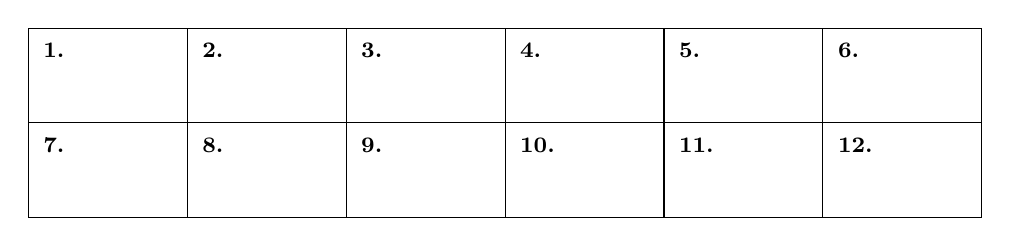
\begin{tikzpicture}
  % ---- 12题：6×2 ----
  \pgfmathtruncatemacro{\cols}{6}
  \pgfmathsetlengthmacro{\boxw}{(\linewidth-0.4pt)/\cols}
  \pgfmathsetlengthmacro{\boxh}{1.2cm}
  \pgfmathsetlengthmacro{\offset}{0.15cm}

  \foreach \num in {1,...,\answerkeytotal} {
    \pgfmathtruncatemacro{\row}{ifthenelse(\num<=\cols,0,1)}
    \pgfmathtruncatemacro{\col}{mod(\num-1,\cols)}
    \pgfmathsetlengthmacro{\x}{\col*\boxw}
    \pgfmathsetlengthmacro{\y}{-\row*\boxh}
    \draw (\x,\y) rectangle ++(\boxw,\boxh);
    \node[anchor=north west, font=\footnotesize, inner sep=1pt] at (\x+\offset,\y+\boxh-\offset) {\textbf{\num.}};
  }
\end{tikzpicture}

\end{flushleft}
}